%*************************************************************************
% Dokument Einstellungen
%*************************************************************************
\documentclass[fontsize=12pt,paper=a4,open=any,parskip=half,
  twoside=false,toc=listof,toc=bibliography,fleqn,leqno,
  captions=nooneline,captions=tableabove,british]{scrbook}
%*************************************************************************
% Importieren von Paketen die benutzt werden
%*************************************************************************
\usepackage[utf8]{inputenc} % load early
\usepackage[T1]{fontenc}    % load early
\usepackage[ngerman]{babel}
\usepackage[autostyle=true]{csquotes}
\usepackage{graphicx, booktabs, float, scrhack}
\usepackage{caption}
\usepackage{listings}
%\usepackage{fancyref}
%\usepackage{showkeys}
\usepackage[svgnames]{xcolor}
\usepackage{amsmath,amssymb}
\usepackage[automark]{scrlayer-scrpage}
\usepackage[backend=biber,style=alphabetic]{biblatex} %,sortcase=false,

%*************************************************************************
% Bibliographies - Zitatquellen
%*************************************************************************
\addbibresource{Projekt.bib}

%*************************************************************************
% Weitere Dokument Einstellungen
%*************************************************************************
\PassOptionsToPackage{hyphens}{url} 
\usepackage[hidelinks]{hyperref}  % load late
\setkomafont{disposition}{\sffamily}
%*************************************************************************
% Dokumentanfang
%*************************************************************************
\begin{document}
%Aktivierung römische Seitenzahlen
\frontmatter

%Titelblatt Einstellungen
\titlehead{% siehe KOMA-Script-Anleitung
  \begin{minipage}[t]{0.65\textwidth}
    \raggedright
    			Frankfurt University of Applied Sciences\\
				Fachbereich 2: Informatik und Ingenieurwissenschaften\\
				Studiengang: Informatik (B.Sc.)\\
  \end{minipage}
  \hfill
  \raisebox{-\dimexpr\totalheight-\ht\strutbox\relax}{
    
\includegraphics[width=5cm]{Bilder/fra-uas}
  }
}

\subject{Projektarbeit}
\title{Software-defined Networking mit Openflow}
\subtitle{}
\author{Mücahit Sagiroglu\\
Matrikelnummer: 1228852\\
James Belmonte\\
Matrikelnummer: 1340604\\
Naghmeh Ghavidel Rostami\\
Matrikelnummer:\\
Tund Trinh\\
Matrikelnummer:\\
}
\date{Vorgelegt am: 1. Februar 2022}
\publishers{Dozent: Maurizio Petrozziello\\
Modul 25: Informatik Projekt\\
Software-defined Networking mit Openflow\\
Wintersemester 2021/2022\\
}

\maketitle
%Eigenständigkeitserklärung
\chapter*{Eigenständigkeitserklärung}
Hiermit erklären wir, dass wir die vorliegende Arbeit eigenständig verfasst, keine anderen als die
angegebenen Quellen und Hilfsmittel verwendet sowie die aus fremden Quellen direkt oder indirekt
übernommenen Stellen/Gedanken als solche kenntlich gemacht haben. Diese Arbeit wurde noch keiner
anderen Prüfungskommission in dieser oder einer ähnlichen Form vorgelegt. Sie wurde bisher auch nicht
veröffentlicht.

Hiermit stimmen wir zu, dass die vorliegende Arbeit von der Prüferin/ dem Prüfer in elektronischer Form
mit entsprechender Software auf Plagiate überprüft wird.

\begin{figure}[H]
	\centering
	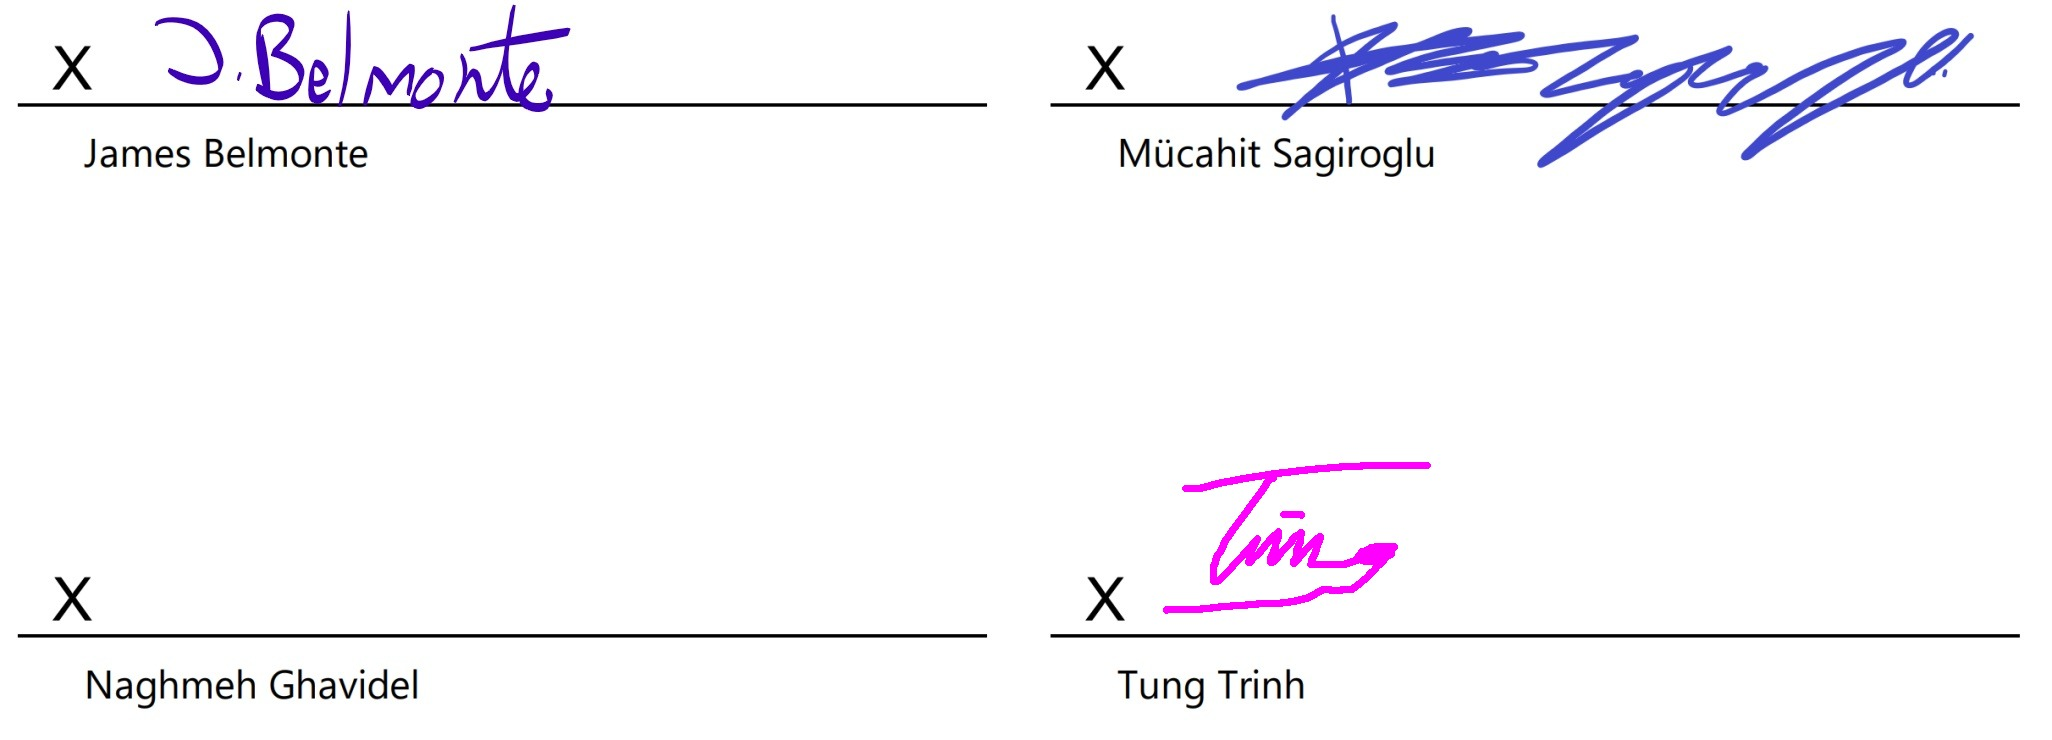
\includegraphics[width=1\linewidth]{Bilder/unterschrift}
\end{figure}

%Inhaltsverzeichnes & Abbildungsverzeichnis & Tabellenverzeichnis
\tableofcontents
\listoffigures
\listoftables
\lstlistoflistings

%Aktivierung arabische Seitenzahlen
\mainmatter % Seite fängt mit 1 an



%Kapitel: Einleitung
\chapter{Einleitung}\label{ch:intro}
Seit der Einführung des ... existiert das ..., welcher, wie der Name ausdrückt, einige ... für .... zur Verfügung stellt.

%Kapitel: Java.Util
\chapter{Kapitel 1}\label{ch:j.u}
Hier kommt Kapitel 1. Aufzählungen gehen so:
\begin{itemize}
 \item Aufzählung 1
 \item Aufzählung 2
 \item Aufzählung 3
 \item ...
\end{itemize}
Hier kann der Text weitergehen.

%Kapitel: Interface
\chapter{Kapitel 2}\label{ch:interfaces}
Hier steht Kapitel 2. Hier kommt ein Listing:
\begin{lstlisting}[language=Java,
					caption={Deklaration eines Interfaces},
					backgroundcolor = \color{lightgray},
					captionpos=b,
					numbers=left,
					keywordstyle=\color{RoyalBlue},
    				rulecolor=\color{black},
   		 			upquote=true, 
					showstringspaces=false,
    				breaklines=true,
    				frame=single,
					aboveskip=2em,
					label={interface-deklaration},
]
public interface Interface1 extends Interface2, Interface3 {
	...
	public int methode(int zahl1, int zahl2);
	...
}
\end{lstlisting}
\captionsetup{justification=centering,margin=2cm}

Hier geht der Text weiter. Und so bindet man ein Figure ein(Bild im Ordner Bilder zu finden):


\begin{figure}[htbp]
 \centering
 
\includegraphics[width=0.6\textwidth]{Bilder/bildname}
 \captionsetup{justification=centering,margin=2cm}
 \caption{Beziehungen von Klassen und Interfaces \autocite{jtpinterface}}
 \label{interface-relation}
\end{figure}

Hier kann der Text weitergehen.


\section{Unterkapitel 1}\label{sec:c.f}
Hier ist ein Unterkapitel (Section). Hier paar Aufzählungen:

\begin{itemize}
 \item public boolean add(E e) 
 \item public boolean remove(Object element)
 \item public int size()
 \item public boolean contains(Object element)
 \item public boolean isEmpty()
\end{itemize}

Text geht weiter..... Hier kommt eine Tabelle:

\begin{table}[htbp]
\caption{Eigenschaften von Vector, PriorityQueue und HashSet}
\label{data-table}
\centering
  \begin{tabular}{l  c  c  c} 
\toprule
    Eigenschaften & Vector & PriorityQueue & HashSet\\ 
\midrule  
    Doppelte Einträge erlaubt:   		& Ja  	&  Ja  	& Nein \\
    Reihenfolge:   						& Ja 	&  Ja 		& Nein \\ 
	Veränderbar:   						& Ja	&  Nein 	& Ja \\ 
	Thread-Safe:   						& Ja 	& Nein 	& Nein\\ 
  \end{tabular}

\end{table}


\section{Unterkapitel 2}\label{ch:vector}
Hier geht der Text weiter. Noch eine Tabelle:

\begin{table}[htbp]
\caption{Eigenschaften der Python Datenstrukturen \autocite{listuple}}
\label{python-data-table}
\centering
  \begin{tabular}{l  c  c  c c} 
\toprule
    Eigenschaften & List & Tuple & Set & Dict\\ 
\midrule  
    	Doppelte Einträge erlaubt:   			& Ja  	&  Ja  		& Nein 	& Keine doppelten Keys\\
    	Reihenfolge:   						& Ja 	&  Ja 		& Nein 	& Ja\\ 
	Veränderbar:   						& Ja	&  Nein 	& Ja 		& Ja\\ 
	Thread-Safe:   						& Ja 	& Ja 	& Ja 		& Ja\\ 
  \end{tabular}

\end{table}

%Kapitel: Fazit
\chapter{Fazit}\label{ch:fazit}
Mit der Hausarbeit sollte eine Übersicht auf das .... gegeben und geschaut werden, ob gleiche oder ähnliche Architekturen in ..... vorhanden sind. Hierzu wurde der Bereich auf die .... und .... eingegrenzt, da das .... sehr umfangreich ist. \par



\printbibliography[title=Literaturverzeichnis]

\end{document}